%%%%%%%%%%%%%%%%%%%%%%%%%%%%%%%%%%%%%%%%%
% Beamer Presentation
% LaTeX Template
% Version 1.0 (10/11/12)
%
% This template has been downloaded from:
% http://www.LaTeXTemplates.com
%
% License:
% CC BY-NC-SA 3.0 (http://creativecommons.org/licenses/by-nc-sa/3.0/)
%
%%%%%%%%%%%%%%%%%%%%%%%%%%%%%%%%%%%%%%%%%

%----------------------------------------------------------------------------------------
%	PACKAGES AND THEMES
%----------------------------------------------------------------------------------------

 \documentclass{beamer}

\mode<presentation> {

% The Beamer class comes with a number of default slide themes
% which change the colors and layouts of slides. Below this is a list
% of all the themes, uncomment each in turn to see what they look like.

%\usetheme{default}
%\usetheme{AnnArbor}
%\usetheme{Antibes}
%\usetheme{Bergen}
%\usetheme{Berkeley}
%\usetheme{Berlin}
%\usetheme{Boadilla}
%\usetheme{CambridgeUS}
%\usetheme{Copenhagen}
%\usetheme{Darmstadt}
%\usetheme{Dresden}
%\usetheme{Frankfurt}
%\usetheme{Goettingen}
%\usetheme{Hannover}
%\usetheme{Ilmenau}
%\usetheme{JuanLesPins}
%\usetheme{Luebeck}
\usetheme{Madrid}
%\usetheme{Malmoe}
%\usetheme{Marburg}
%\usetheme{Montpellier}
%\usetheme{PaloAlto}
%\usetheme{Pittsburgh}
%\usetheme{Rochester}
%\usetheme{Singapore}
%\usetheme{Szeged}
%\usetheme{Warsaw}

% As well as themes, the Beamer class has a number of color themes
% for any slide theme. Uncomment each of these in turn to see how it
% changes the colors of your current slide theme.

%\usecolortheme{albatross}
%\usecolortheme{beaver}
%\usecolortheme{beetle}
%\usecolortheme{crane}
%\usecolortheme{dolphin}
%\usecolortheme{dove}
%\usecolortheme{fly}
%\usecolortheme{lily}
%\usecolortheme{orchid}
%\usecolortheme{rose}
%\usecolortheme{seagull}
%\usecolortheme{seahorse}
%\usecolortheme{whale}
%\usecolortheme{wolverine}

%\setbeamertemplate{footline} % To remove the footer line in all slides uncomment this line
%\setbeamertemplate{footline}[page number] % To replace the footer line in all slides with a simple slide count uncomment this line

%\setbeamertemplate{navigation symbols}{} % To remove the navigation symbols from the bottom of all slides uncomment this line
}
\usepackage{graphicx} % Allows including images
\usepackage{booktabs} % Allows the use of \toprule, \midrule and \bottomrule in tables
\usepackage{amsmath}
\usepackage{mathrsfs}
\bibliographystyle{ieeetr}
%----------------------------------------------------------------------------------------
%	TITLE PAGE
%----------------------------------------------------------------------------------------

\title[Assignment]{Assignment: 3-Achieving Usable and Privacy-assured Similarity Search over Outsourced Cloud Data} % The short title appears at the bottom of every slide, the full title is only on the title page

\author{Author} % Your name
\institute[DLUT] % Your institution as it will appear on the bottom of every slide, may be shorthand to save space
{
Dalian University of Technology \\
\textit{Assignment of System Security} % Your institution for the title page
\medskip % Your email address
}
\date{\today} % Date, can be changed to a custom date

\begin{document}

\section{Introduction}
\begin{frame}
\titlepage % Print the title page as the first slide
\end{frame}

\begin{frame}
	\frametitle{Overview} % Table of contents slide, comment this block out to remove it
	\tableofcontents % Throughout your presentation, if you choose to use \section{} and \subsection{} commands, these will automatically be printed on this slide as an overview of your presentation
\end{frame}
\begin{frame}
	\frametitle{Introduction of the Paper}
	\bibliography{myreference}    
\end{frame}

\begin{frame}
 \frametitle{Introduction of the Paper}
 \begin{block}{Purpose}
  Solve the problem of secure and efficient fuzzy search over encrypted outsourced cloud data
  \end{block}
  
  \begin{block}{Measures}
  	\begin{itemize}
  		\item Suppressing technique 
  		\item Building a private trie-traverse searching index
  	\end{itemize}
  \end{block}
  
  \begin{block}{Performance}
	  Correctly achieves the defined similarity search functionality with \textbf{\textcolor{red}{constant}}  searching time!
  \end{block}
  
  
\end{frame}


%----------------------------------------------------------------------------------------
%	PRESENTATION SLIDES
%----------------------------------------------------------------------------------------

%------------------------------------------------
\section{Background} % Sections can be created in order to organize your presentation into discrete blocks, all sections and subsections are automatically printed in the table of contents as an overview of the talk
%------------------------------------------------
\begin{frame}
	\frametitle{System and Threat Model}
	\begin{figure}
	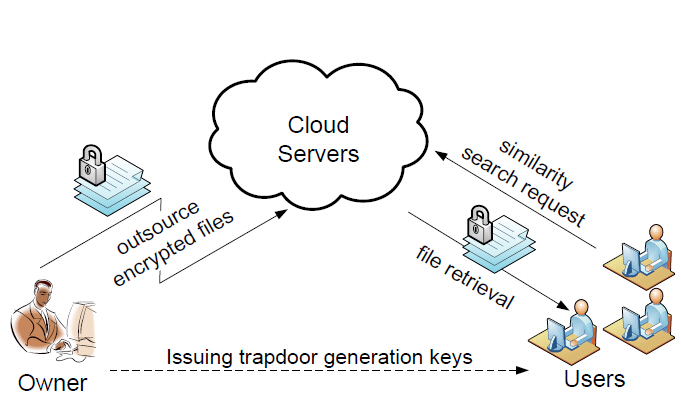
\includegraphics[width=0.6\linewidth]{fig1.jpg}
	\caption[1]{Architecture of similarity keyword search over outsourced cloud data}
	\end{figure}
		\begin{itemize}
			\item data owner: the individual/enterprise customer,who has a collection of $n$ data files $C = ({F_1},{F_2}, \ldots ,{F_n})$ to be stored in the cloud server.
			\item $W = \left\{ {{w_i},{w_w}, \ldots ,{w_p}} \right\}$ is denoted as a predefined set of distinct keywords in $C$
		\end{itemize}
\end{frame}
%\subsection{Subsection Example} % A subsection can be created just before a set of slides with a common theme to further break down your presentation into chunks
\begin{frame}
	\frametitle{System and Threat Model}
	\begin{itemize}
		\item Files are encrypted before outsourced
		\item The data owner will distribute search request\textcolor{red}{(trapdoor) generation keys $sk$} to authorized users.(Assume that the authorization will be done appropriately)
		\item An authorized user uses \textcolor{red}{trapdoor generation key} to generate a search request via some \textcolor{red}{one-way function} to search word $w$, and submit it to the cloud.
		\item The cloud then performs the search over the data
		collection $C$ without decryption and sends back all encrypted files containing the specific keyword $w$, denoted as $FI{D_w}$.
		\item \textcolor{blue} {The
		similarity keyword search scheme returns the closest possible results based on aforementioned measures.}
		\item At last, the user decrypts files they received from the cloud.
	\end{itemize}
\end{frame}

\begin{frame}
	\frametitle{Assumption: Honest-but-curious clound server}
    To ensure the securely similarity searching schema:
    \begin{columns}[t] 
    \column{.3\textwidth}
    \begin{block}{Honest}
    	Correctly follows the designated protocol specification
    \end{block}
    \column{.5\textwidth}
        \begin{alertblock}{Curious}
        	Infer and analyze the message flow received during the protocol so as to learn additional information
        \end{alertblock}
    \end{columns}
    \begin{columns}
    \column{.8\textwidth}
    \begin{exampleblock}{}
        We follow the security definition
        deployed in the traditional  \textcolor{red} {searchable symmetric encryption(SSE)}
    \end{exampleblock}
\end{columns}
\end{frame}

\begin{frame}
	\frametitle{Notations}
	\begin{description}
		\item[$C$]the file collection to be outsourced, denoted as a set of $n$ data files $C = ({F_1},{F_2}, \ldots ,{F_n})$.
		\item[$W$]the distinct keywords extracted from file collection $C$, denoted as a set of $m$ words $W = \left\{ {{w_i},{w_w}, \ldots ,{w_p}} \right\}$.
		\item[$\cal I$]the index built for privacy-assured similarity search.
		\item[${T_w}$] the trapdoor generated by a user as a search request of input keyword $w$ via some one-way transformation.
		\item[${S_{w,d}}$] similarity keyword set of $w$, where $d$ is the similarity threshold according to a certain similarity metrics.
		\item[$FI{D_{{w_i}}}$]the set of identifiers of files in $C$ that contain keyword ${{w_i}}$.
		\item[$f(key, \cdot ),g(key, \cdot )$]pseudorandom function (PRF), defined	as: ${\{ 0,1\} ^*} \times key \to {\{ 0,1\} ^{\ell }}$.
		\item[$Enc(key, \cdot ),Dec(key, \cdot )$]symmetric key based semantic secure encryption/decryption function.
	\end{description}
\end{frame}
\section{Suppression Technique}
\begin{frame}
	\frametitle{Edit Distance}
	\begin{columns}
	\end{columns}
	\begin{block}{Quantitative measurement}
		The edit distance $ed({w_1},{w_2})$ between two words ${w_1}$ and ${w_2}$ is the \textcolor{red}{mininum} number of \textcolor{red}{primitive operations}, including \textcolor{blue}{character insertion, deletion} and \textcolor{blue}{substitution}, necessary to transform one of them into the other.
	\end{block}
	
	\begin{block}{Similarity keyword set}
		Given a keyword $w$, we let ${S_{w,d}}$ denote its similarity set of words, such that any $w' \in {S_{w,d}}$ satisfies \textcolor[rgb]{0.1,0.6,0.3}{$ed(w,w') \le d$}  for a certain integer $d$.
	\end{block}
	
	\begin{exampleblock}{Example}
		Consider the keyword $w_0=$\textit{CENSOR}\\
		a words set W = \{\textit{CESOR},\textit{CENSER},\textit{CEANSOR}\}\\
		for any $w' \in W$,$ed({w_0},w') \le 1$ holds,\\
		i.e. $w' \in {S_{{w_0},1}}$ and $W \subseteq {S_{{w_0},1}}$
	\end{exampleblock}
\end{frame}

\begin{frame}
	\frametitle{Building Similarity Keyword Sets}
	\begin{columns}
		\column{.45\textwidth}
		\begin{alertblock}{Straightforward approach}
			Simply \textcolor{red}{enumerating} all possible words $w{'_i}$ satisfying the similarity
			criteria $ed({w_i},w{'_i}) \le d$
		\end{alertblock}
		\begin{alertblock}{}
		For the keyword $w_0=$\textit{CENSOR},
		consider just one substitution operation with charaters on first character.\\
		There are 26 items \{\textit{AENSOR},\textit{BENSOR}, \ldots ,\textit{YENSOR},\textit{ZENSOR}\} \\
		So ${S_{{w_0},1}}$ will be $[6 + (6 + 1)] \times \textcolor{red}{26} + \textcolor{green}1$
		\end{alertblock}
		\column{.5\textwidth}
		\begin{block}{Suppression technique}
			Consider only the \textcolor{blue}{positions} of the primitive edit operations.Specifically, we use a \textcolor{blue}{wildcard ‘*’ }to
			denote all three operations of character insertion, deletion and
			substitution at any position.
		\end{block}
		
		\begin{block}{}
			Now,\\
 ${{{S}}_{SENSOR,1}} = $ \{\textit{SENSOR}, \textit{*SENSOR, *ENSOR},\textit{S*ENSOR}, \textit{S*NSOR}, \ldots, \textit{SENSO*R}, \textit{SENSO*}, \textit{SENSOR*}\}.
			Size can be reduced to ${S_{{w_0},1}}$ will be $[6 + (6 + 1)] \times \textcolor{blue}{1} + \textcolor{green}1$
		\end{block}
	\end{columns}
\end{frame}

\begin{frame}
	\frametitle{Building Similarity Keyword Sets}
	\begin{figure}
		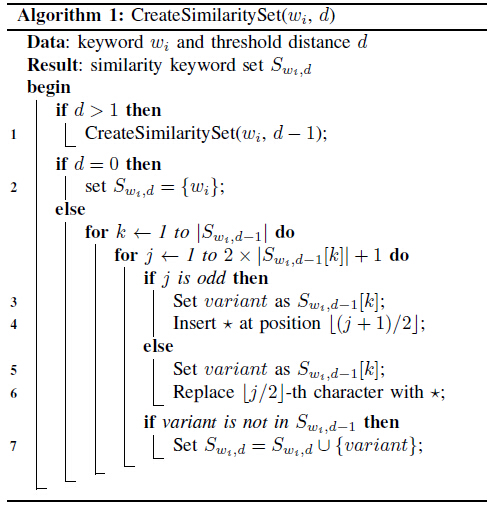
\includegraphics[width=0.4\linewidth]{algo1.jpg}
	\end{figure}
	The size of ${S_{{w_i},d}}$ will be ${\cal O}(\textcolor{blue}{\ell ^d})$,opposing to ${\cal O}(\textcolor{blue}{{\ell ^d}} \times \textcolor{red}{26^d})$ obtained in the \textcolor{red}{straightforward approach}.
\end{frame}

\begin{frame}
	\frametitle{Generating Searching Request}
	\begin{theorem}
		The intersection of the similarity sets \textcolor{blue}{${S_{{w_i},d}}$} and \textcolor{red}{${S_{w,d}}$} for keyword \textcolor{blue}{$w_i$} and  search input \textcolor{red}{$w$} is not empty if and only if $ed(\textcolor{red}{w},\textcolor{blue}{w_i}) \le d$.
	\end{theorem}
	
	\begin{proof}
		\begin{itemize}
			\item Completeness(i.e. $ed(\textcolor{red}{w},\textcolor{blue}{w_i}) \le d \to \textcolor{red}{S_{{w_i},d}} \cap \textcolor{blue}{S_{w,d}} \ne \emptyset $ ):
			\begin{itemize}
				\item $\textcolor{red}{w} \to \textcolor{blue}{{w_i}}$ need at most $d$ primitive operations.\\the result after these operations is marked as $w^*$
				\item $w^*$ is naturally in \textcolor{red}{${S_{w,d}}$} 
				\item $w^*$ can be transformed into \textcolor{blue}{${w_i}$}, so it must be in \textcolor{blue}{${S_{{w_i},d}}$} 
				\item $w' \in \textcolor{blue}{S_{{w_i},d}} \cap \textcolor{red}{S_{w,d}}$
			\end{itemize}
		\end{itemize}
	\end{proof}
\end{frame}

\begin{frame}
	\frametitle{Generating Searching Request}
	\begin{proof}
		\begin{itemize}
			\item Soundness(i.e. $\textcolor{blue}{S_{{w_i},d}} \cap \textcolor{red}{S_{w,d}} \ne \emptyset  \to ed(\textcolor{red}{w},\textcolor{blue}{w_i}) \le d$) \\
			\begin{description}
				\item[${w^*}$]the common element in $\textcolor{blue}{S_{{w_i},d}} \cap \textcolor{red}{S_{w,d}}$
			\end{description}
			\begin{enumerate}
				\item ${w^*}$ does not contain any wildcard *,\\
				then ${w^*} =\textcolor{red}{ w} =\textcolor{blue}{ w'}$,and $ed(\textcolor{red}{w},\textcolor{blue}{w'}) = 0 \le d$
				\item ${w^*}$ does contain some wildcard *(at most d *'s),\\
				change * in $w^*$ back to the character in \textcolor{red}{$w$} and \textcolor{blue}{$w_i$},\\
				denote the result as \textcolor{red}{$w{'^*}$} and \textcolor{blue}{$w{'_i}^*$} with both sharing $d-1$ different *'s.\\
				$\textcolor{red}{w{'^*}} \to \textcolor{blue}{w{'_i}^*}$ need at most one primitive operation.\\
				So, $ed(\textcolor{red}{w{'^*}},\textcolor{blue}{w{'_i}^*}) \le 1$\\
				$ \Rightarrow ed(\textcolor{red}{w},\textcolor{blue}{{w_i}}) \le d$
				
			\end{enumerate}
		\end{itemize}
	\end{proof}
\end{frame}

\section{The Basic Scheme}

\begin{frame}
	\frametitle{The Basic Scheme}
	\begin{block}{}
		\begin{description}
			\item[$\tau $]the maximum size of the similarity keyword set $S_{{w_i},d}$ for ${w_i} \in W$, i.e.,$\tau  = \max {\left\{ {\left| {{S_{{w_i},d}}} \right|} \right\}_{{w_i} \in W}}$ where $\left| W \right| = p$.
		\end{description}
	\end{block}
		\begin{exampleblock}{Prepocessing phase(the owner)}
			\begin{enumerate}
				\item  picks random key $x$,$y$,and builds index ${\cal I} = {\left\{ {f(x,w{'_i}),Enc(s{k_{w{'_i}}},FI{D_{{w_i}}})} \right\}_{w{'_i} \in {S_{{w_i},d}},1 \le i \le p}}$, where secret key $s{k_{w{'_i}}} = g(y,w{'_i})$
				\item insert extra $\tau \left| W \right| - \left| {\cal I} \right|$ dummy entries(using random values) in $\cal I$ for padding.
				\item randomly shuffles $\cal I$, outsources $\cal I$, encrypted $C$ to cloud.
			\end{enumerate}
		\end{exampleblock}
\end{frame}

\begin{frame}{The Basic Scheme}
	\begin{alertblock}{Searching phase(the user)}
		\begin{enumerate}
			\item generates ${{S_{w,d}}}$ from input $w$ via Algorithm 1 and derives ${T_{w'}} = (f(x,w'),g(y,w'))$ for each $w' \in {S_{w,d}}$
			\item generates $\tau  - \left| {{S_{w,d}}} \right|$ dummy trapdoors by randomly choosing $j$ from ${\left\{ {f(x,j),g(y,j)} \right\}_{1 \le j \le \tau \left| W \right| - \left| {\cal I} \right|}}$
			\item Cloud server compares all received trapdoors $\left\{ {f(x,w')} \right\}$(and $\left\{ {f(x,j)} \right\}$) with ${\cal I}$ uses the corresponding $\left\{ {g(y,w')} \right\}$ to decrypt the matched entries,  and returns the union of file identifiers, ${\left\{ {FI{D_{{w_i}}}} \right\}_{ed(w,{w_i}) \le d}}$.
			\item The user retrieves and decrypts the files of interest.
		\end{enumerate}
	\end{alertblock}
	\begin{block}{Improvement}
		Storage and search cost is ${\cal O}(\tau \left| W \right|)$.\\
		Bloom Filters can be introduced in to reduce the searching cost to  ${\cal O}( \left| W \right|)$
	\end{block}
\end{frame}

\section{The Symbol-based Trie-Traverse Searching Schema}

\begin{frame}{The Symbol-based Trie-Traverse Searching Schema}
	\begin{block}{All similar words in the trie can be found by a depth-first search}
		Construct a multi-way tree for storing the similarity keyword elements over a finite symbol set.All trapdoors sharing a common prefix have a common node.	The root is associated with an empty set. 
	\end{block}
	\begin{columns}
		\column{0.45\textwidth}
    \begin{figure}
      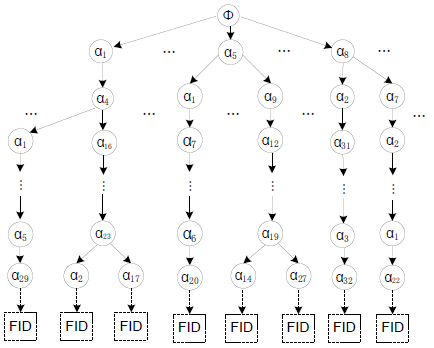
\includegraphics[width=\textwidth]{fig2.jpg}
      \caption{The depth of the tree is $l/\theta$}
    \end{figure}
    \column{.45\textwidth}
    \begin{exampleblock}{}
    	\begin{itemize}
    		\item Assume $\Delta  = \left\{ {{\alpha _i}} \right\}$ is a predefined symbol set.
    		\item $\left| \Delta  \right| = {2^\theta }$
    		\item each symbol ${\alpha _i} \in \Delta $ is denoted by a $\theta$-bit binary vector.
    		\item $l$ is the output length of one-way function $f(key, \cdot )$.
    	\end{itemize}
    	
    \end{exampleblock}
    \end{columns}
\end{frame}

\begin{frame}{The Symbol-based Trie-Traverse Searching Schema}
		\begin{columns}
			\column{.49\textwidth}
			\begin{exampleblock}{Preprocessing phase(the owner)}
		\begin{enumerate}
			\item 	computes ${f(x,w{'_i})}$ for each ${w{'_i} \in {S_{{w_i},d}}}$,${1 \le i \le p}$ together with dummy entries.
			\item divides them into symbols as ${\alpha _{{i_1}}} \cdots {\alpha _{{i_{l/\theta }}}}$ from $\Delta$.
			\item builds up a trie ${G_W}$ covering all ${w_i} \in W$.
			\item attaches ${\left\{ {Enc(s{k_{w{'_i}}},FI{D_{{w_i}}})} \right\}_{w{'_i} \in {S_{{w_i},d}},1 \le i \le p}}$ to $G_W$,\\outsourced it\\ with encrypted collection $C$ to the cloud.
			
			
		\end{enumerate}
			\end{exampleblock}
			
			\column{.44\textwidth}
			\begin{alertblock}{Searching phase(the user)}
			 \begin{enumerate}
			 	\item sends a set of $\tau $ trapdoors(research request): ${\left\{ {{T_{w'}}} \right\}_{w' \in {S_{w,d}}}}$ and $\tau  - \left| {w' \in {S_{w,d}}} \right|$ dummy trapdoors.
			 	\item the cloud server divides each $f(x,w')$ into a sequence of symbols from $\Delta$. Perform the search over the trie $G_W$.
			 	\item decrypts matches entries via $g(y,w')$ and return ${\left\{ {FI{D_{{w_i}}}} \right\}_{ed(w,{w_i}) \le d}}$ to the user.
			 \end{enumerate}
			\end{alertblock}
		\end{columns}
\end{frame}

\begin{frame}{The Symbol-based Trie-Traverse Searching Schema}
	\begin{figure}
		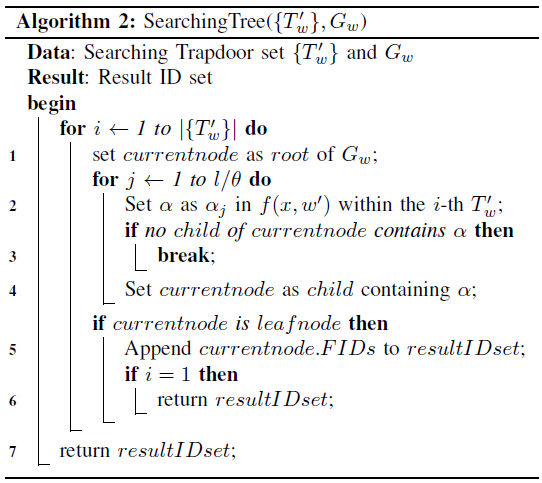
\includegraphics[width=0.5\textwidth]{algo2.jpg}
	\end{figure}
	The search cost at the server side is only \textcolor{red}{${\cal O}(1)$}(a \textcolor{red}{constant} related to $l/\theta$)
\end{frame}

\section{Scheme Evaluation}

\begin{frame}{Scheme Evaluation}
	\begin{table}
		\begin{tabular}{l l l l}
			\toprule
			{} & \textbf{SSE} & \textbf{Basic} & \textbf{Trie-traverse}\\
			\midrule
			 \textbf{Preprocessing} & ${\cal O}(\left| W \right|)$ & ${\cal O}(\tau \left| W \right|)$ & ${\cal O}(\tau \left| W \right|)$ \\
			 \textbf{Index size} & ${\cal O}(\left| W \right|)$ & ${\cal O}(\tau \left| W \right|)$ & ${\cal O}(\tau \left| W \right|)$ \\
			 \textbf{Search cost} & ${\cal O}(1)$ & ${\cal O}(\tau \left| W \right|)$ & \textcolor{red}{${\cal O}(1)$}  \\
			 \textbf{Similarity search} & No & Yes & No \\
			\bottomrule
		\end{tabular}
		\caption{Comparison of SSE schemes}
	\end{table}

\end{frame}

\section{Experiment}

\begin{frame}{Experiment}
		\begin{block}{Experiment Design}
			\begin{itemize}
				\item A real data set: RFC, 5,731 plaintext files, 277MB
				\item C programming language 
				\item Local workstation
				\item Cloud side:Amazon Elastic Computing Cloud(EC2)
			\end{itemize}
		\end{block}
		\begin{exampleblock}{Note}
			In our experiment the dominant factor affecting the performance is th number of \textcolor{red}{unique keywords} to be indexed, not the \textcolor[rgb]{0.1,0.7,0.2}{file collection size}.
		\end{exampleblock}
\end{frame}

\begin{frame}{Cost for Generating Similarity Keyword Set}
	\begin{figure}
        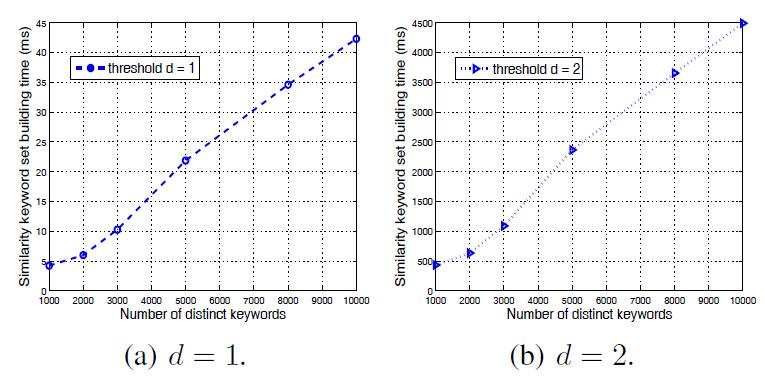
\includegraphics[width=0.8\textwidth]{subfig1.jpg}
        \caption{Similarity set construction time using wildcard-based approach with different choices of edit distance $d$}
	\end{figure}
	\begin{block}{}
		The construction time increases \textcolor{blue}{linearly} with the number of keywords.
	\end{block}
\end{frame}

\begin{frame}{Cost For Building Searchable Index}
    \begin{columns}
    	\column{.45\textwidth}
	\begin{figure}
		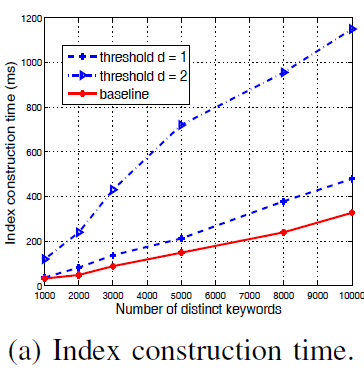
\includegraphics[width=\textwidth]{subfig2.jpg}
		\caption{Time cost for searchable index construction with different choices of edit distance $d$}
	\end{figure}
	\column{.5\textwidth}
	    \begin{alertblock}{}
	    	For completeness, we also include the index building time of existing SSE as a \textcolor{red}{baseline} for comparison here.
	    \end{alertblock}
	    \begin{exampleblock}{}
	    	The whole index construction is just a one-time cost and can be conducted off-line
	    \end{exampleblock}
	\begin{block}{}
		Similar to the similarity keyword set construction, the index construction time increases \textcolor{blue}{linearly} with the number of distinct keywords.
	\end{block}
	\end{columns}
\end{frame}

\begin{frame}{Cost For Building Searchable Index}
	\begin{columns}
		\column{.45\textwidth}
	\begin{figure}
		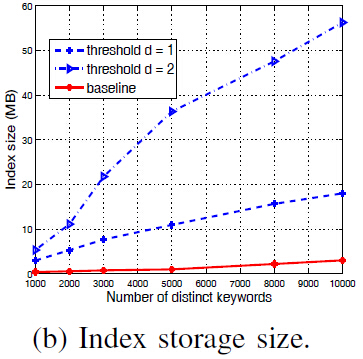
\includegraphics[width=\textwidth]{subfig3.jpg}
		\caption{Storage cost for searchable index construction with different choices of edit distance $d$}	
	\end{figure}
	\column{.5\textwidth}
	\begin{exampleblock}{}
		Again, our approach consumes more storage space than the baseline due to the \textcolor[rgb]{0.1,0.7,0.2}{multi-way tree structure} and the \textcolor[rgb]{0.1,0.7,0.2}{additional entries} in the index corresponding to the similarity keywords
	\end{exampleblock}
	\begin{block}{}
		But can be deemed as \textcolor{blue}{reasonable} cost of supporting similarity search
	\end{block}
	\begin{alertblock}{}
		"average keyword length" also \textcolor{red}{sightly} influence the time and space cost of building searchable index.
	\end{alertblock}
	\end{columns}
\end{frame}

\begin{frame}{Cost For Searching the Index}
	\begin{figure}
		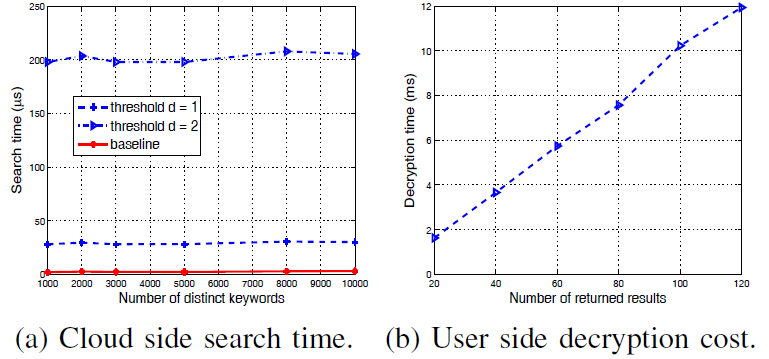
\includegraphics[width=.75\textwidth]{subfig4.jpg}
		%\caption{Evaluation for search cost and file retrieval}
	\end{figure}
	\begin{block}{}
		The proposed  mechanism cost \textcolor{blue}{constant} search time.
	\end{block}
	\begin{exampleblock}{}
		Cost for results retrieval and decryption is plainly determined by the \textcolor[rgb]{0.1,0.7,0.2}{number} of retrieved results
	\end{exampleblock}
\end{frame}


%------------------------------------------------
\section{The End}
\begin{frame}
\Huge{\centerline{Thanks}}
\end{frame}

%----------------------------------------------------------------------------------------

\end{document} 